\section{\scshape Sensors and environments modeling}
\subsection*{Sensors modeling}
\begin{frame}{Depth sensors modeling}
	\begin{itemize}
		\item Modeling of 8 different types of depth sensors
		\begin{itemize}
			\item Time of Flight (ToF) sensor
			\begin{itemize}
				\item Kinect XBox One
			\end{itemize}
			\item Structured light sensors
			\begin{itemize}
				\item Asus Xtion Pro Live
				\item Ensenso N35
				\item Intel RealSense SR300
				\item Kinect XBox 360
				\item Orbbec Astra
			\end{itemize}
			\item Stereo vision sensors
			\begin{itemize}
				\item MultiSense S7
				\item ZED stereo camera
			\end{itemize}
		\end{itemize}
		\item Pinhole camera model coupled with OpenGL color rendering and depth buffer allows to specify the sensors:
		\begin{itemize}
			\item Resolution (width and height in pixels)
			\item Field of view (vertical and horizontal FOV in radians)
			\item Minimum and maximum measurement range (near and far z-buffer clipping planes in meters)
			\item Sensor acquisition rate (number of image acquisitions per second in hertz)
		\end{itemize}
	\end{itemize}
\end{frame}


\begin{frame}{Depth sensors modeling}
	\begin{figure}
		\centering
		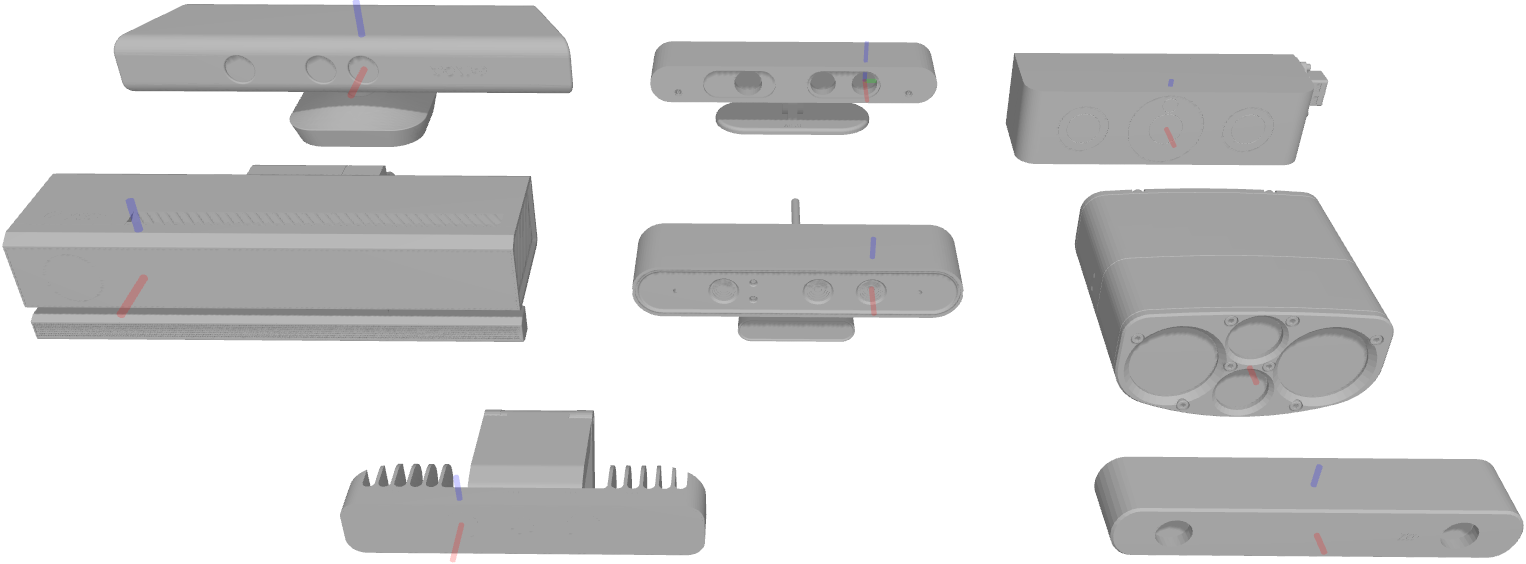
\includegraphics[width=\textwidth]{sensors/sensors-gray-with-links}
		\caption{Sensors 3D CAD models with the display of the depth image coordinate frames using the ROS convention of x-y-z -> forward-left-up (horizontally from top left to bottom right: Kinect XBox 360, Asus Xtion Pro Live, Ensenso N35, Kinect XBox One, Orbbec Astra, MultiSense S7, Intel RealSense SR300, ZED stereo camera)}
	\end{figure}
\end{frame}


\subsection*{Environments modeling}
\begin{frame}{Environments modeling}
	\begin{itemize}
		\item Modeling of 4 different test environments
			\begin{itemize}
				\item 1 for active perception, with hand occlusions
				\item 1 for bin picking with minimal occlusions
				\item 1 for bin picking with significant occlusions
				\item 1 for multiple object bin picking with several occlusions
			\end{itemize}
		\item Modeling of 3 bin picking objects
		\begin{itemize}
			\item Starter motor (target object for bin picking)
			\item Alternator (for bin picking occlusions)
			\item Differential gearbox (for bin picking occlusions)
		\end{itemize}
		\item Modeling of 2 support objects
		\begin{itemize}
			\item Trolley with shelves
			\item Large stacking box
		\end{itemize}
		\item Target objects use a special surface material that ignores light effects (such as light shading and shadows) and have a specific color (pure green) that will be used for sensor data segmentation. It was used .stl CAD models for 3D rendering and .ply point clouds for 3D data processing
	\end{itemize}
\end{frame}


\begin{frame}{Active perception environment}
	\begin{figure}
		\centering
		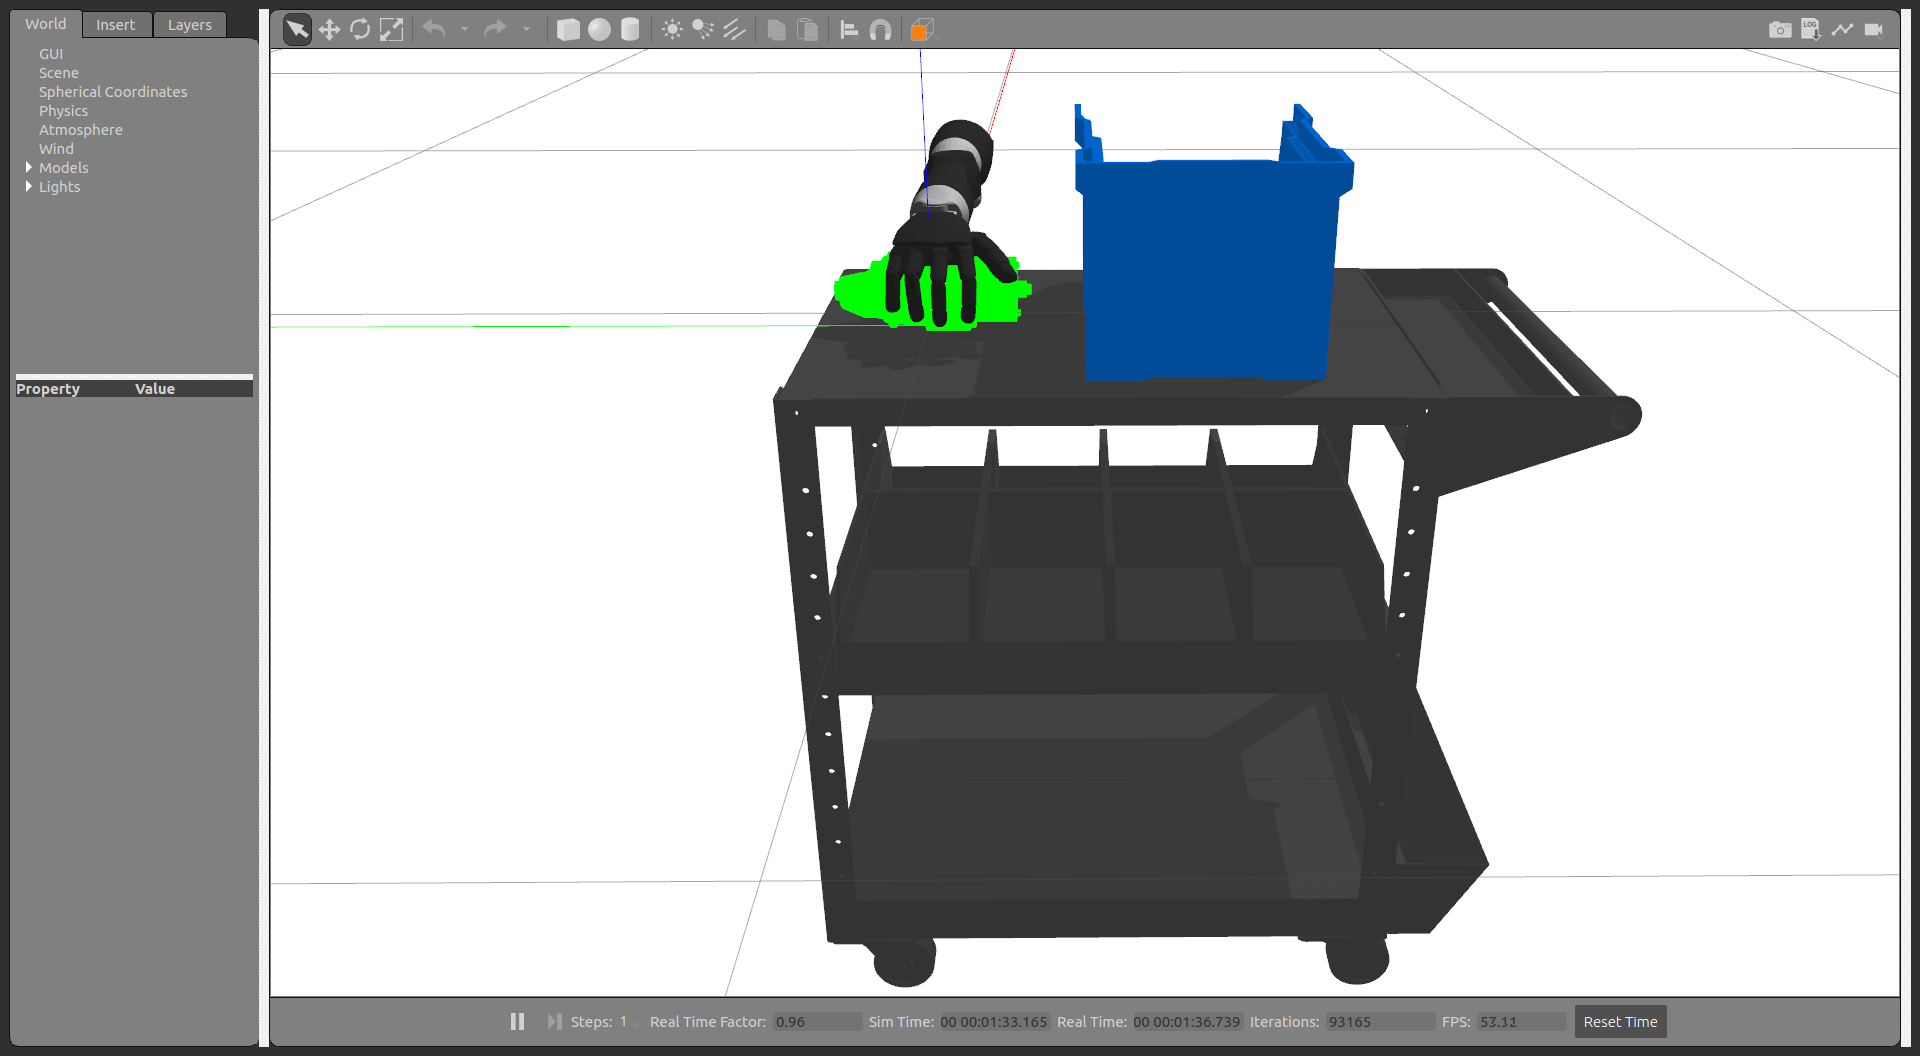
\includegraphics[height=.25\textwidth]{environments/active-perception/gazebo-back}
		\includegraphics[height=.25\textwidth]{environments/active-perception/gazebo-top}\\
		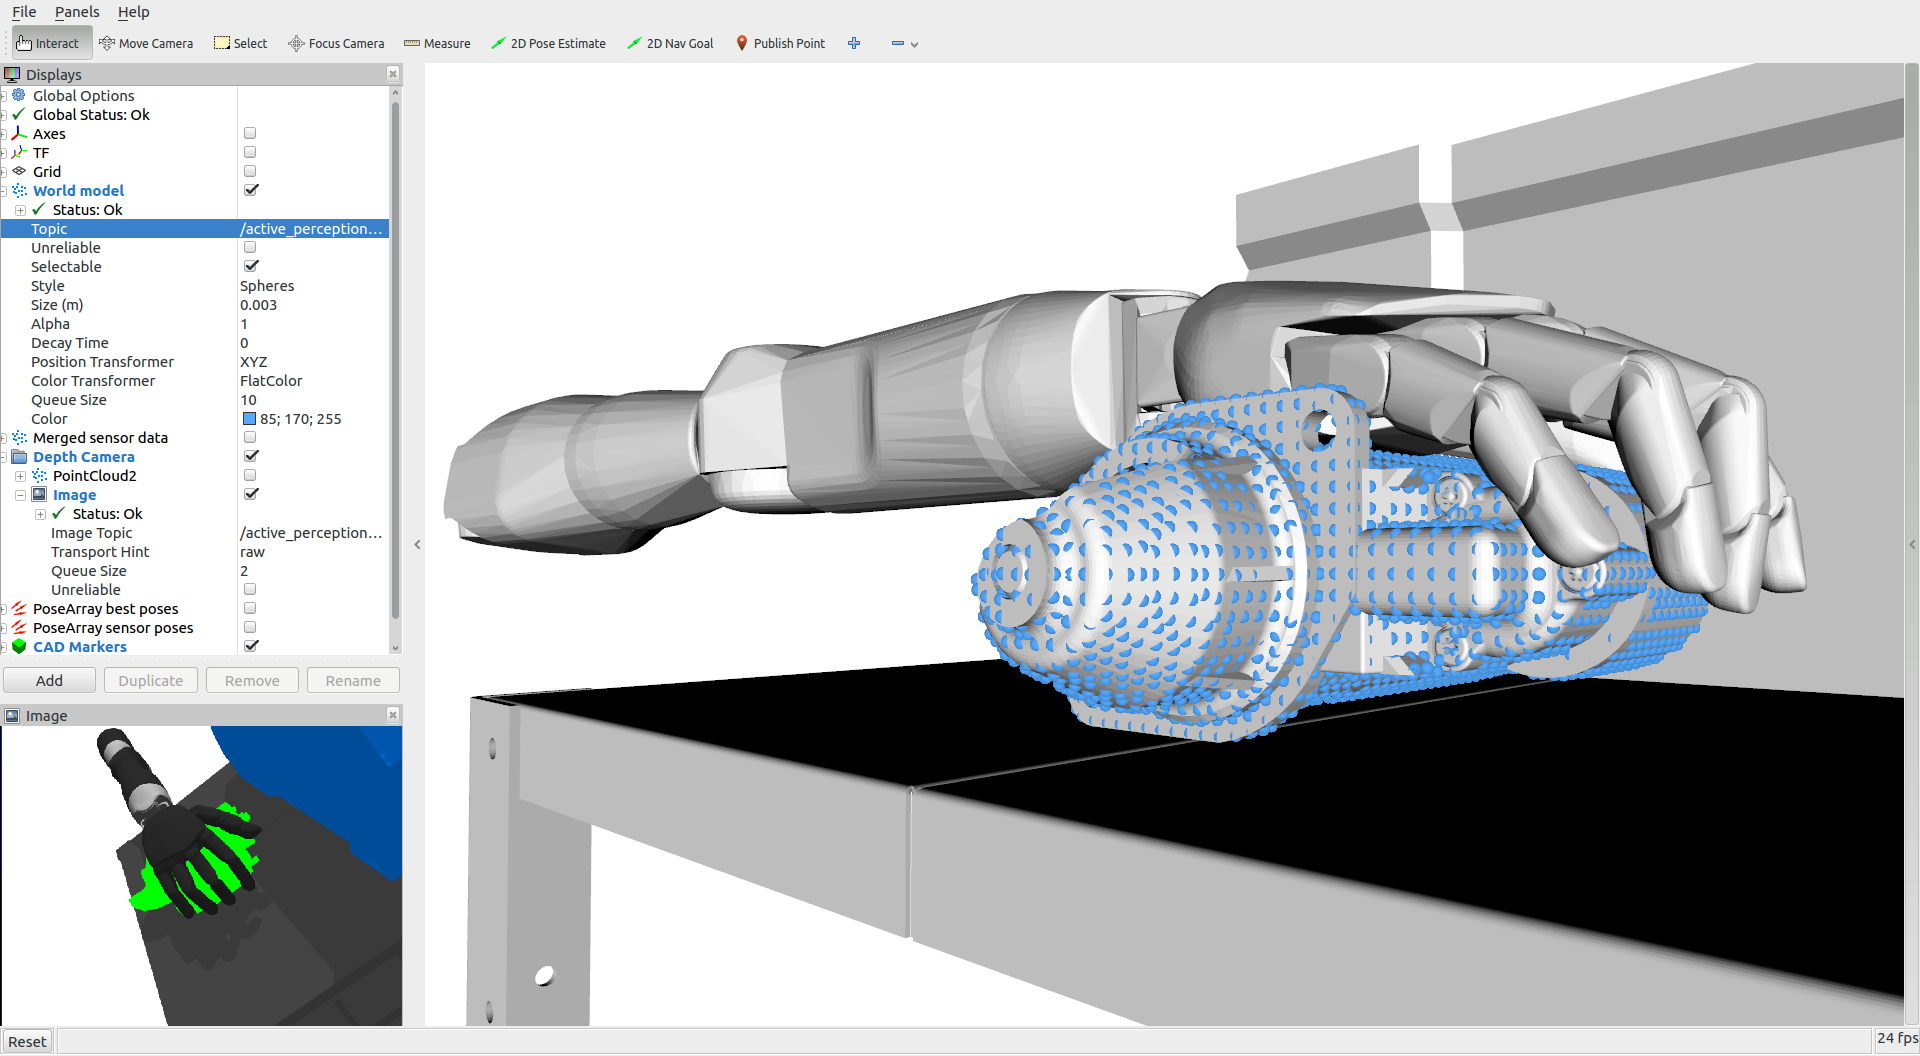
\includegraphics[height=.25\textwidth]{environments/active-perception/rviz-back-left}
		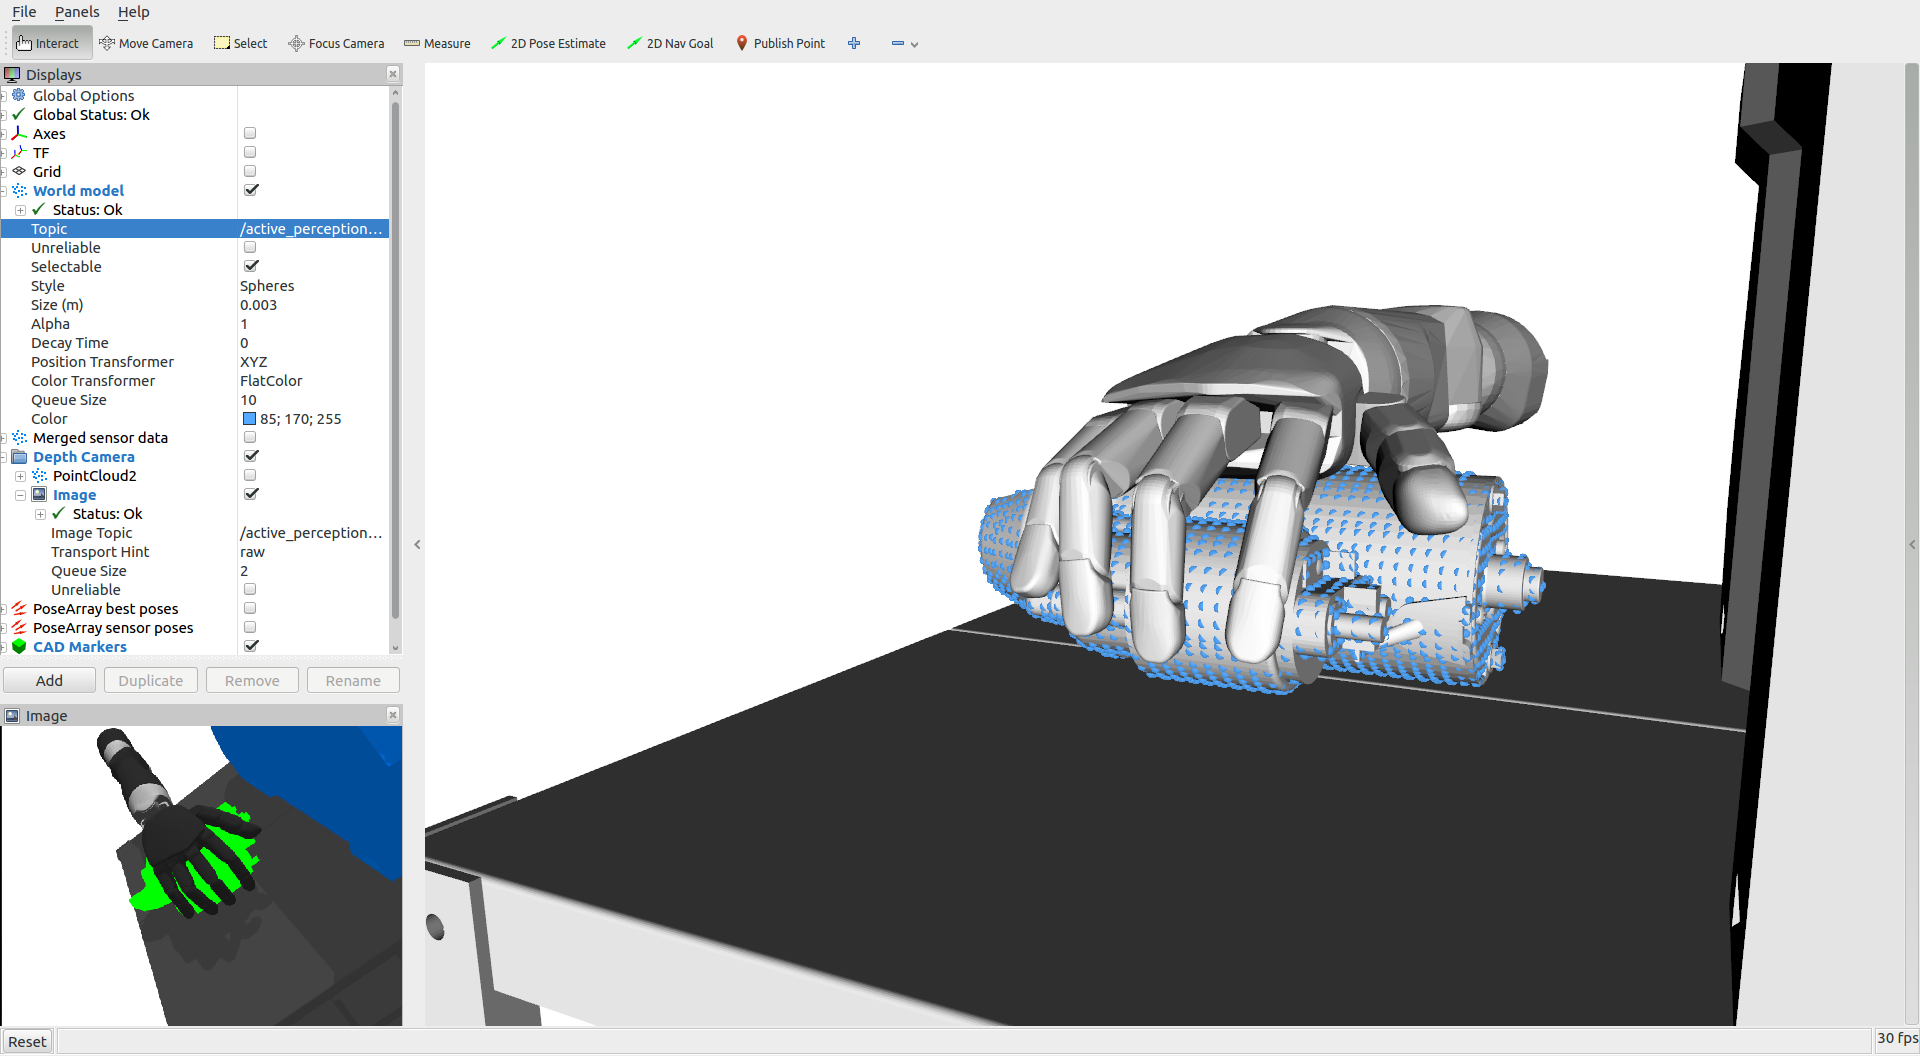
\includegraphics[height=.25\textwidth]{environments/active-perception/rviz-back-right}
		\caption{Active perception environment renderings from Gazebo with target objects in green (top images) and associated CAD model point clouds displayed as blue spheres in Rviz (bottom images)}
	\end{figure}
\end{frame}


\begin{frame}{Bin picking environment}
	\begin{figure}
		\centering
		\includegraphics[height=.25\textwidth]{environments/bin-picking/gazebo-front}
		\includegraphics[height=.25\textwidth]{environments/bin-picking/gazebo-top}\\
		\includegraphics[height=.25\textwidth]{environments/bin-picking/rviz-front}
		\includegraphics[height=.25\textwidth]{environments/bin-picking/rviz-top}
		\caption{Bin picking environment renderings from Gazebo with target objects in green (top images) and associated CAD model point clouds displayed as blue spheres in Rviz (bottom images)}
	\end{figure}
\end{frame}


\begin{frame}{Bin picking with occlusions environment}
	\begin{figure}
		\centering
		\includegraphics[height=.25\textwidth]{environments/bin-picking-with-occlusions/gazebo-front}
		\includegraphics[height=.25\textwidth]{environments/bin-picking-with-occlusions/gazebo-top}\\
		\includegraphics[height=.25\textwidth]{environments/bin-picking-with-occlusions/rviz-front}
		\includegraphics[height=.25\textwidth]{environments/bin-picking-with-occlusions/rviz-top}
		\caption{Bin picking with occlusions environment renderings from Gazebo with target objects in green (top images) and associated CAD model point clouds displayed as blue spheres in Rviz (bottom images)}
	\end{figure}
\end{frame}


\begin{frame}{Multiple bin picking with occlusions environment}
	\begin{figure}
		\centering
		\includegraphics[height=.25\textwidth]{environments/multiple-bin-picking-with-occlusions/gazebo-front}
		\includegraphics[height=.25\textwidth]{environments/multiple-bin-picking-with-occlusions/gazebo-top}\\
		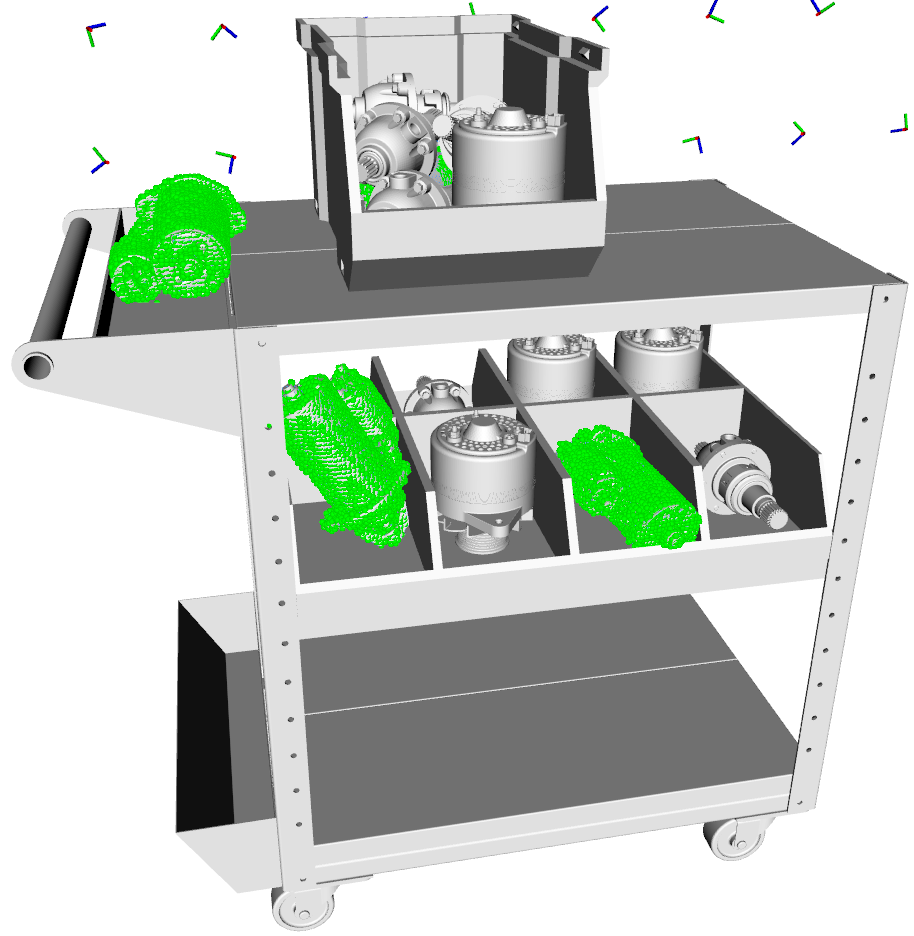
\includegraphics[height=.25\textwidth]{environments/multiple-bin-picking-with-occlusions/rviz-front-corner}
		\includegraphics[height=.25\textwidth]{environments/multiple-bin-picking-with-occlusions/rviz-top}
		\caption{Multiple bin picking with occlusions environment renderings from Gazebo with target objects in green (top images) and associated CAD model point clouds displayed as blue spheres in Rviz (bottom images)}
	\end{figure}
\end{frame}
